\chapter{Specification}\label{chap:specification}

Below ``$\log$'' means ``$\log_2$'', ``$\Vert$'' is string concatenation, all hash values are 32-byte. The type of tree used is a complete binary hash tree (i.e., a complete Merkle tree).

\section{Primitives}

\gravity requires three hash functions, which all return 32-byte hash
values:

\begin{itemize}

\item \hashx takes input values of any length. We use \textbf{SHA-256} as \hashx.

\item \hashy takes input values of 32 bytes. We use \textbf{Haraka-256} with 6 rounds as \hashy.

\item \hashz takes input values of 64 bytes. We use \textbf{Haraka-512} with 6 rounds as \hashz.

\end{itemize}
The Haraka versions are the v2~\cite{haraka}.

\gravity also uses \textbf{AES-256-CTR} as a deterministic generator of pseudorandom bytes.



\section{Parameters}

\gravity signature schemes are defined by three parameters:

\begin{itemize}

\item The \textbf{set size} $T$, which must be a power of two.

\item The \textbf{subset size} $K$, which must be lower than $T$.

\item The \textbf{number of subtrees} $C$, which must be a power of two and strictly lower than $T$.

\end{itemize}

These parameters determine:

\begin{itemize}

\item The \textbf{public key size}, equal to $32C$ bytes.

\item The \textbf{signature size}, equal to $32\times (K + K(\log T- \log C)+1)$ bytes.

\end{itemize}

$T$ and $K$ together determine the security and signature length, while $C$ determines the public key and signature lengths but not security. 

The choice of $T$ and $K$ depends on the target security security level and on the maximum number of messages to be signed.
The security level for a given $(T,K)$ is discussed in \S\ref{sec:attacks}.

The choice of $C$ is mostly a trade-off between the public key size (higher with a higher $C$) and the  signature size (smaller with a higher $C$).
The optimal value of $C$ for a given $(T,K)$ is discussed in \S\ref{sec:tradeoff}.


\section{Key Generation}

A secret key \sk is a random 64-byte value, viewed as two 32-byte values $\sk_1\Vert\sk_2=\sk$.

A public key \pk is derived from a secret key's $\sk_1$ as follows:

\begin{enumerate}

\item Expand \sk into $T$ 32-byte \emph{subkeys} $\ek_0, \ek_1, \dots, \ek_{T-1}$, by taking the first $32T$ bytes generated with AES-256-CTR keyed with $\sk_1$ and with a 16-byte counter initialized to \hex{0000\dots0000}.

\item Hash each subkey to obtain $T$ values $L_i=\hashy(\ek_i)$, $i=0,\dots,T-1$, which will be the leaves of the tree.

\item Compute $\pk = \pk_0, \cdots, \pk_{C}$ as the $C$ nodes on level $\log C$ of the binary hash tree with leaves $L_0, \dots, L_{T-1}$, computing $\hashz(L_0\Vert L_1)$, $\hashz(L_2\Vert L_3)$, and so on.

\end{enumerate}

Step 1 requires $32T$ bytes from \drbg, step 2 requires $T$ calls to $\hashy$, and step 3 requires $T - C$ calls to $\hashz$.

The value $\log C$ can be seen as the ``cut-off'' level of the tree.

The $\sk_2$ component of the secret key is not used in key generation, but only when signing a message.


\section{Subset Generation}\label{sec:subsetgen}

The core component of \gravity is its \emph{subset generation function}, which picks $K$ distinct values in $0, 1, \dots, T-1$ given a 32-byte \emph{signature seed} $S$ and $H = \hashx(M)$, the 32-byte hash of the message.

Subset generation works like this:

\begin{itemize}

\item Compute the \emph{subset seed} $D=\hashz(S\Vert H)$.

\item Generate pseudorandom bits from \drbg keyed with $D$ and with a 16-byte counter initialized to \hex{0000\dots0000}.

\item Parse the pseudorandom stream as a sequence of 4-byte big-endian unsigned integers $N_0, N_1, N_2, \dots$, where each integer is reduced modulo $T$ (since $T$ is a power of two, the distribution remains uniform)

\item Determine the $K$ distinct values $V_0,\dots,V_{K-1}$  as follows: $V_0=N_0$; $V_1$ is the first $N_i, i>0$ such that $N_i\neq V_0$; third value is the first subsequent $N_i$ distinct from both $V_0$ and $V_1$, and so on.

\end{itemize}

\section{Signing a Message}

Given a secret key $\sk=\sk_1\Vert \sk_2$ and a message $M$, \gravity computes a signature $\sig$ as follows:

\begin{enumerate}

\item Generate a subset of indices $V_0, V_1,\dots,V_{K-1}$ as per \S\ref{sec:subsetgen}, using $S=\hashz(\sk_2 \Vert \hashx(M))$ as signature seed. Initialize the signature with the 32-byte $S$.

\item Expand $\sk_1$ into $T$ 32-byte \emph{subkeys} $\ek_0, \ek_1, \dots, \ek_{T-1}$ in the same manner as for public key generation.

\item Append $K$ subkeys to the signature in order to have $\sig= S \Vert \ek_{V_0}\Vert \ek_{V_1}\Vert \cdots \Vert \ek_{V_{K-1}}$.

\item Compute the binary hash tree up to level $1 + \log C$ like for public key generation, but recording the \emph{authentication paths} for each of the $K$ leaves from the subset, as follows:
\begin{enumerate}
\item Hash each subkey to obtain leaves hashes $L_i=\hashx(\ek_i)$, $i=0,\dots,T-1$.
\item Append to $S$ the leaf value to be hashed together with $L_{V_0}$, then the leaf value to be hashed together with $L_{V_1}$, and so on until $L_{V_{K-1}}$.
\item Compute the parent node of each consecutive pair of leaves by doing $\hashz(L_0\Vert L_1)$, $\hashz(L_2\Vert L_3)$, and so on. Append to $S$ the sibling hash value for each of the $K$ parents of a subkey, from $V_0$ to $V_{K-1}$; $K$ hashes are thus appended to $S$.
\item Iterate step (c) for upper levels of the tree, appending sibling nodes to $S$ to form $K$ authentication paths, until level $1 + \log C$ (that is, one level deeper than the level of the subtrees' roots in the public key).
\end{enumerate}
\end{enumerate}
The signature $\sig$ eventually contains, in this order: the signature seed, the $K$ hashes from step 3, and the $K(\log T - \log C)$ hashes from step 4.

Step 1 requires one call to $\hashx$, two calls to $\hashz$, and at least $4K$ bytes from \drbg; step 2 requires $32T$ bytes from \drbg; step 4.a requires $T$ calls to $\hashy$, then iterating step 4.b-d requires $T-C$ calls to $\hashz$.


\begin{figure}
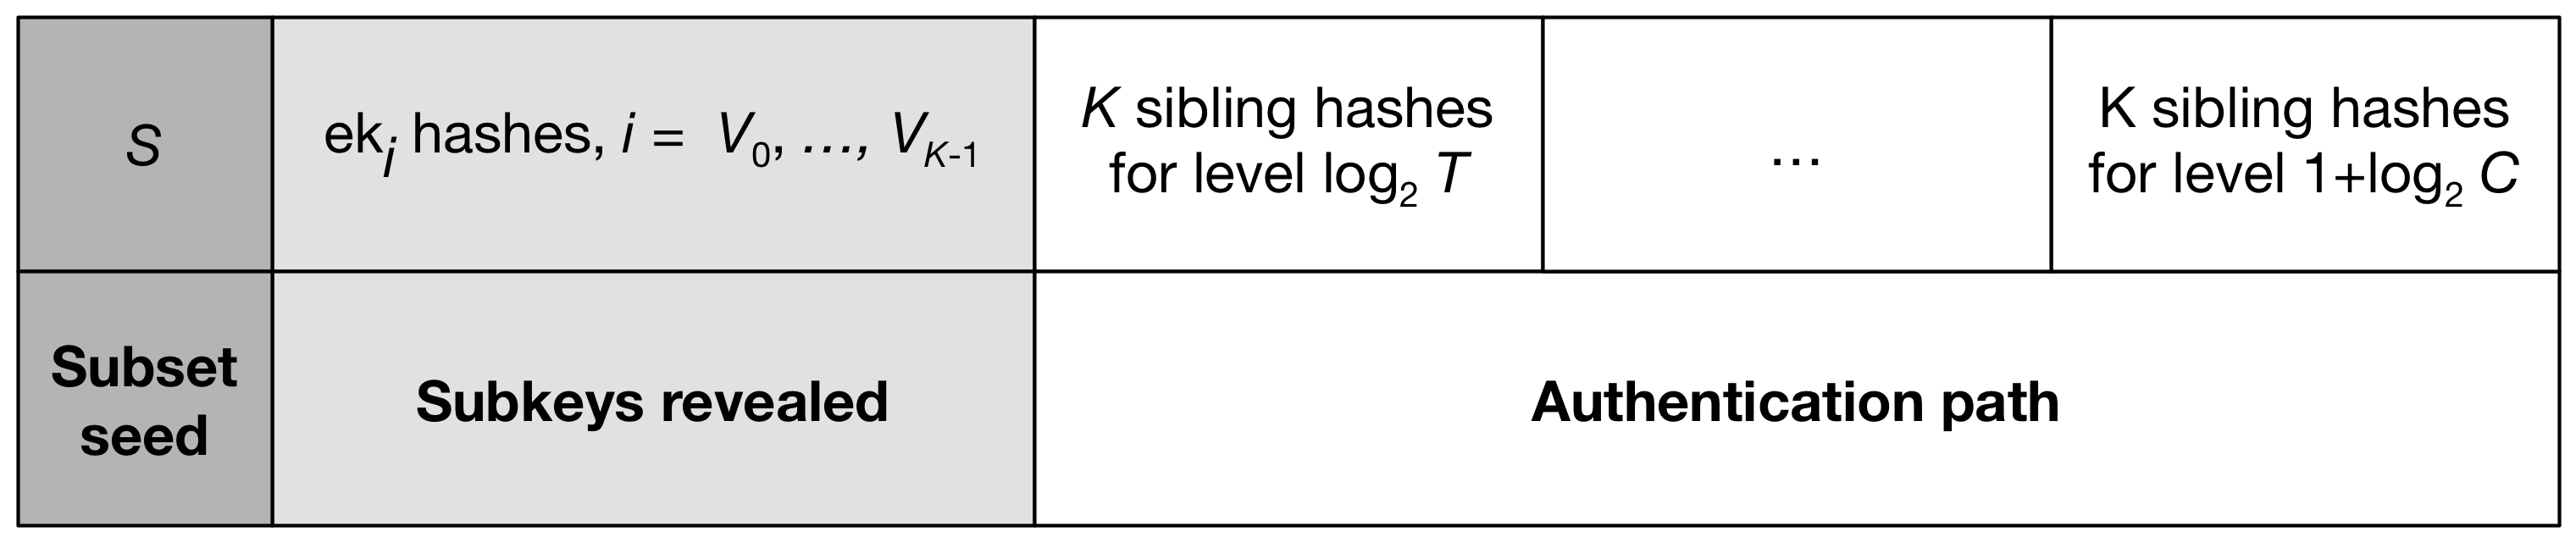
\includegraphics[width=16cm]{sig}
\caption{Content of a signature.}
\end{figure}

\section{Verifying a Signature}

Given a public key \pk and a message $M$, \gravity verifies a signature $\sig$ as follows:

\begin{enumerate}

\item Generate a subset of indices $V_0, V_1,\dots,V_{K-1}$ as per \S\ref{sec:subsetgen}, using the first 32 bytes of \sig as a signature seed.

\item For each of the $K$ indices:
\begin{enumerate}

\item Retrieve the subkey from the signature, where the subkey of index $V_i$ is the $i$th 32-byte string in the signature.

\item Using the authentication path in the signature (every other $K$ hash after the signature seed), compute parent nodes up to level $\log C$.

\item Check if the subtree root found at level $\log C$ is the same as in the public key.

\end{enumerate}
\item Verification of $\sig$ is successful only and only if all $K$ verifications succeeded.
\end{enumerate}

Step 1 requires one call to $\hashx$ and one call to $\hashz$, and at least $4K$ bytes from \drbg; step 2 requires $K$ calls to $\hashy$ and $K (\log T- \log C)$ calls to $\hashz$.


\begin{figure}
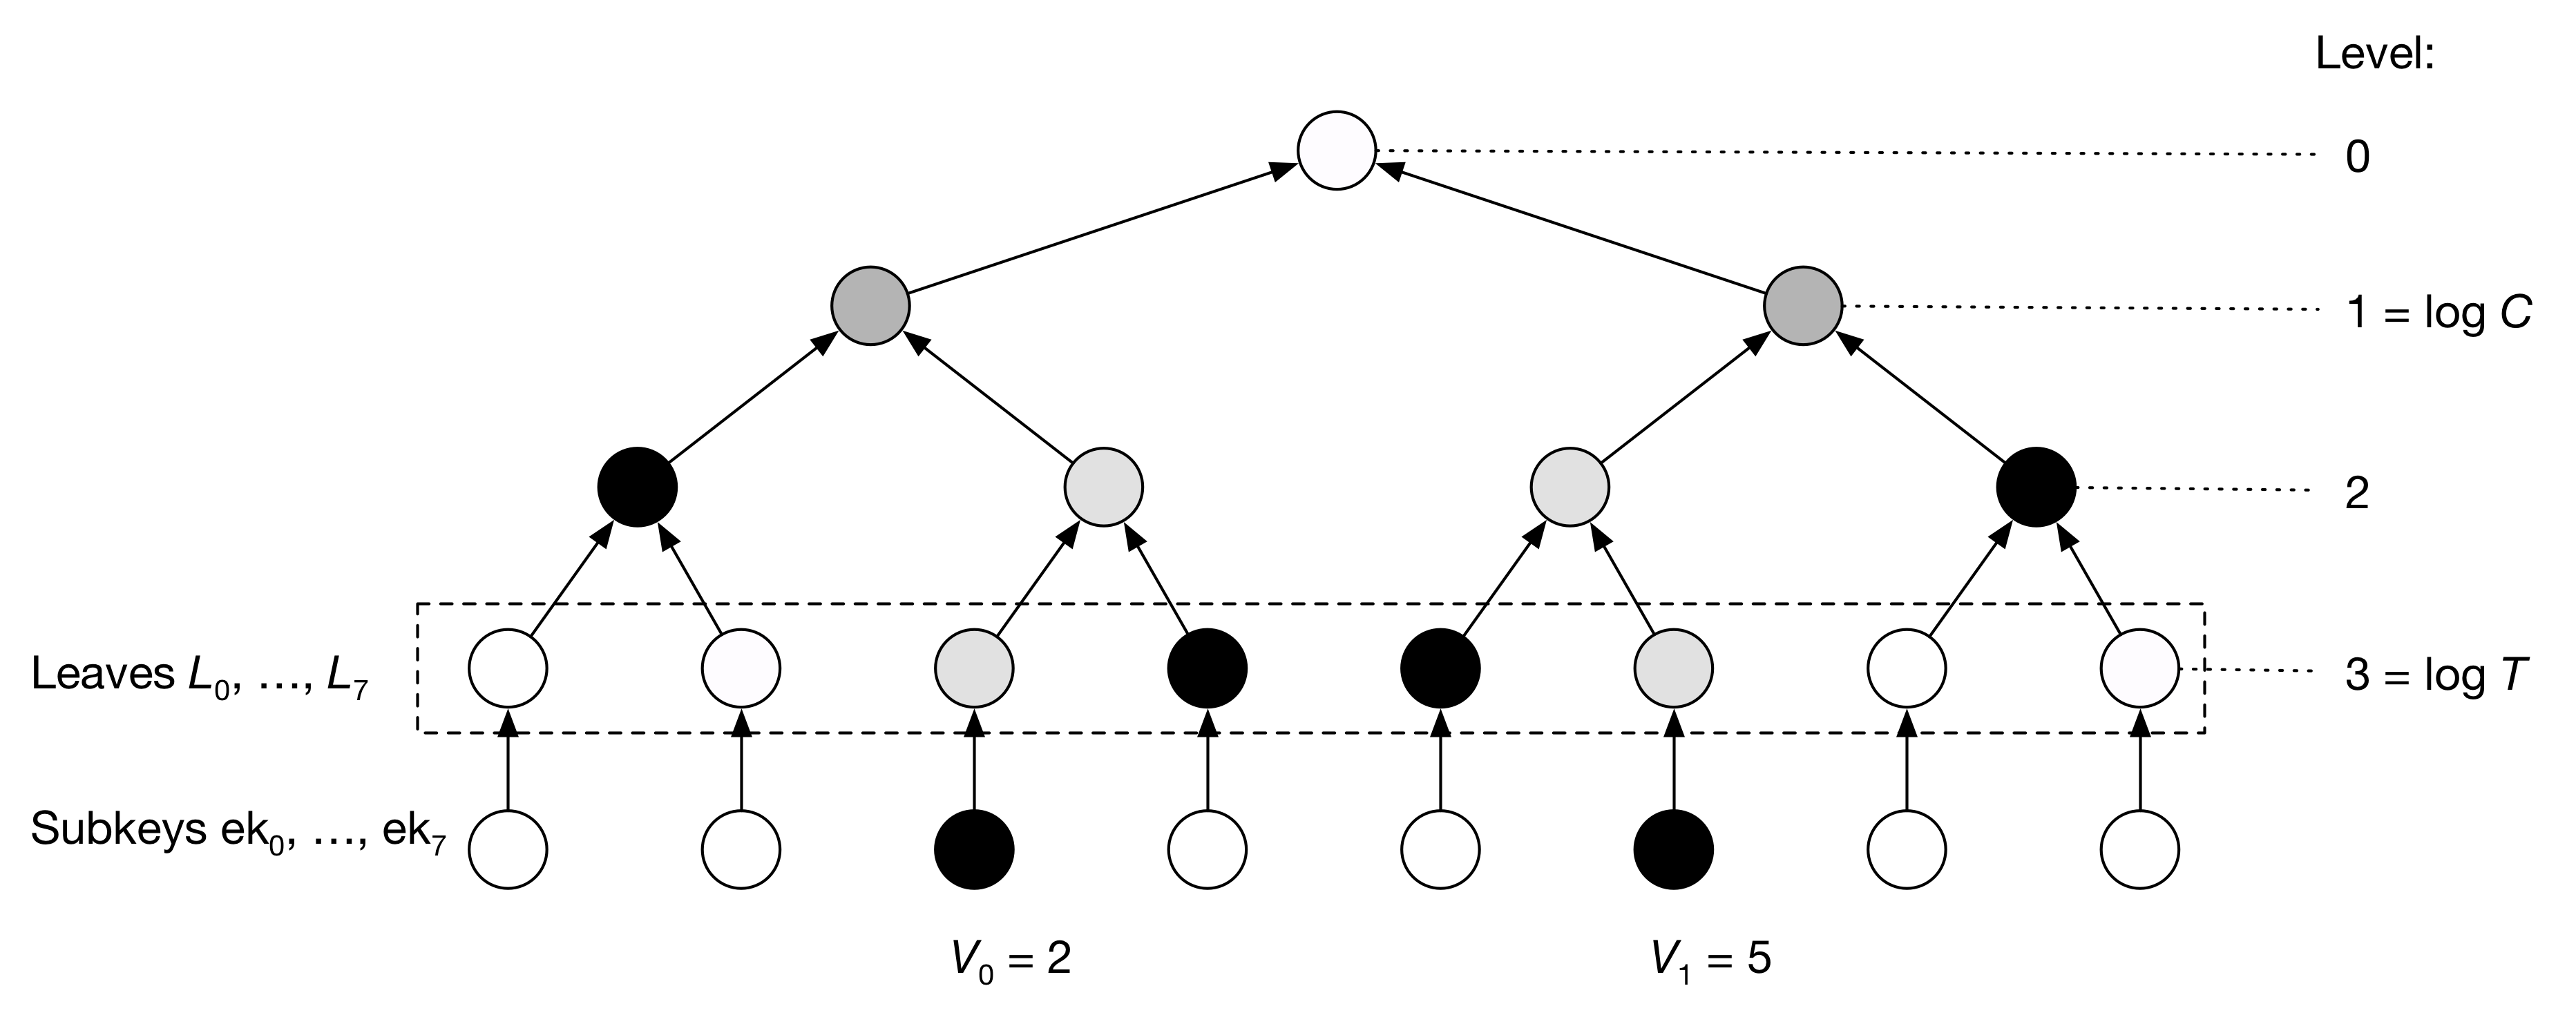
\includegraphics[width=16cm]{tree}
\caption{Binary hash tree of a signature, with a set of $T=8$ hashes (thus a tree depth of $\log T=3$), a subset of $K=2$ hashes, $C=2$ subtrees (thus their two respective roots in the public key), and subset of indexes $V_0=2, V_1=5$. The nodes in black are part of the signature, the nodes in pale grey are computed during the verification, and the nodes in dark grey are part of the public key.
}
\end{figure}

\section{Proposed Instances}

See Table~\ref{tab:instances}.

\begin{table}
\centering 
\begin{tabular}{c|ccc|c|ccc}
\toprule
\multirow{2}{*}{ID} & \multicolumn{3}{c|}{Parameters} & Messages & \multicolumn{3}{c}{Byte length} \\
& $T$ & $K$ & $C$ & limit & Sig & Pub & Priv \\
\midrule
S & $2^{17}$ & 54 & $2^{6}$ & 100 & $\num{20768}$ & 2048 & 64 \\
M & $2^{18}$ & 62 & $2^{7}$ & 300 & $\num{23840}$ & 4096 & 64 \\
L & $2^{19}$ & 64 & $2^{7}$ & 600 & $\num{26656}$ & 4096 & 64 \\
\bottomrule
\end{tabular}
\caption{Proposed \gravity instances, expected to provide 128-bit pre- and post-quantum security.}
\label{tab:instances}
\end{table}
